\subsection{UC5 - Visualizzazione Errore}
\label{sub:uc5}

\begin{figure}[h]
    \centering
    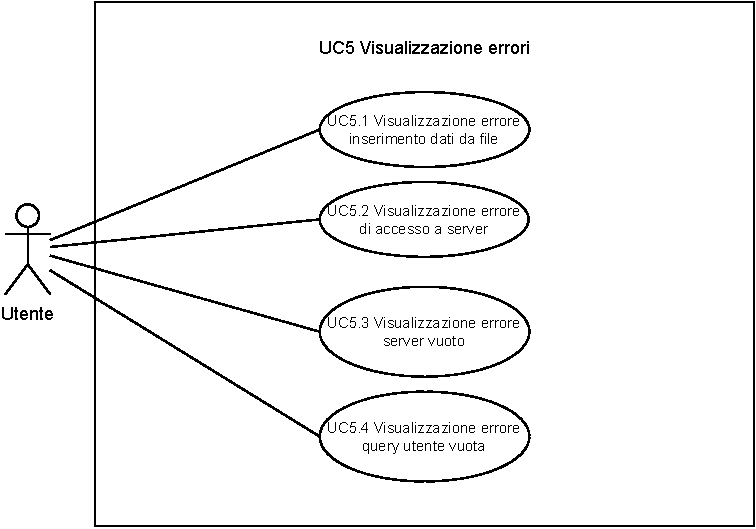
\includegraphics[width=0.7\textwidth]{componenti/casi-duso/diagrammi/UC5.pdf}
    \caption{Diagramma rappresentante UC5}
    \label{fig:UC5}
\end{figure}

\begin{itemize}
    \item \textbf{Descrizione}: Viene visualizzato un messaggio di errore relativo al fallimento di una specifica operazione.

    \item \textbf{Attore primario}: Utente.
    
    \item \textbf{Precondizione}:   Un'operazione fallisce

    \item \textbf{Postcondizione}:  Viene visualizzato un messaggio di errore.
    
    \item \textbf{Scenario Principale}:
    \begin{enumerate}
        \item Viene visualizzato il messaggio di errore.
        \item L'utente conferma di aver preso visione e viene reindirizzato alla home di HD Viz.
    \end{enumerate}

\end{itemize}

%TODO: Cambiare numerazione? Al momento ha senso da una parte ma non è giustificata qui visto che sottocasi non sono veri e propri.

\subsubsection{UC5.1 - Visualizzazione errore inserimento dati da file}
\label{ssub:uc5.1}
\begin{itemize}
    \item \textbf{Descrizione}: All'utente viene mostrato un messaggio d'errore al reperimento
                                dei dati dal file e continua ad utilizzare 
                                il software senza aver correttamente caricato un dataset valido.

    \item \textbf{Attore primario}: Utente.
    
    \item \textbf{Precondizione}:   Il caricamento di dati dal file.

    \item \textbf{Postcondizione}:  Viene visualizzato un messaggio di errore sul reperimento dei 
                                    dati che lo avvisa della mancata formazione di un dataset per il
                                    corretto utilizzo di HD Viz.

\end{itemize}


\subsubsection{UC5.2 - Visualizzazione errore di accesso a server}
\label{ssub:uc5.2}
\begin{itemize}
    \item \textbf{Descrizione}: All'utente viene mostrato un messaggio d'errore di accesso
                                al server al quale HD Viz si dovrebbe connettere, la creazione del dataset viene quindi interrotta.

    \item \textbf{Attore primario}: Utente.
    
    \item \textbf{Precondizione}:   L'apertura della connessione con il server fornito dall'utente fallisce.

    \item \textbf{Postcondizione}:  Viene visualizzato un messaggio di errore sull'apertura della connessione 
                                    con il server e della mancata formazione di un dataset per il corretto utilizzo di HD Viz.

\end{itemize}



\subsubsection{UC5.3 - Visualizzazione errore server vuoto}
\label{ssub:uc5.3}
\begin{itemize}
    \item \textbf{Descrizione}: Dopo aver aperto una connessione con un server HD Viz stabilisce non esserci
                                un database valido al reperimento dati per la creazione del dataset, la creazione
                                del dataset viene quindi interrotta.

    \item \textbf{Attore primario}: Utente.
    
    \item \textbf{Precondizione}:   Il server al quale HD Viz si è connesso è vuoto o i suoi database sono vuoti.

    \item \textbf{Postcondizione}:   Viene visualizzato un messaggio di errore sulla validità del server per il reperimento
                                    dei dati e della mancata formazione di un dataset per il corretto utilizzo di HD Viz.


\end{itemize}


\subsubsection{UC5.4 - Visualizzazione errore query utente vuota}
\label{ssub:uc5.4}
\begin{itemize}
    \item \textbf{Descrizione}: Messaggio relativo all'esecuzione di una query utente su server che restituisce 
                                un set di dati vuoto e
                                perciò la creazione del dataset risulta impossibile e viene interrotta.

    \item \textbf{Attore primario}: Utente.
    
    \item \textbf{Precondizione}:   La query eseguita su server restituisce un set di dati vuoto.

    \item \textbf{Postcondizione}:   Viene visualizzato un messaggio di errore sulla validità del risultato della query 
                                        in quanto vuota non permette la formazione di un dataset corretto per l'uso di HD Viz.


\end{itemize}